\chapter{Background}\label{ch:background}

In this section, the background to this thesis is discussed.
Its aim is to give context to the project that is implemented in addition to specific technical knowledge.
The context of this work is mostly DevOps as it heavily uses implementations of DevOps practices, such as CI/CD tools which are explained in section~\ref{sec:devops-and-agile-programming}.
Testing as a concept exists in software engineering since the beginning and deeper insights are given in section~\ref{sec:testing}.
The DTF, briefly mentioned in section~\ref{ch:introduction} implements theoretical concepts of similarity-based variability testing, which is picked up on in section~\ref{sec:similarities}.
Finally, virtualization of applications and a technology building on top of it, Kubernetes, are described in section~\ref{sec:virtualization} and section~\ref{sec:kubernetes}.

\section{DevOps and agile programming}\label{sec:devops-and-agile-programming}

All things start with Agile programming.
Different practices have emerged since the writing of the agile manifesto~\cite{AgileManifesto} in 2001.
Extreme programming, Scrum and Kanban are only a few examples of such practices~\cite{ADecadeOfAgileMethodologies}.
All of them with the goal of increasing the velocity of software development and the speed at which a project can change into different directions.
These agile practices are more and more adopted in the industry~\cite{BecomingAgileTogether} and taught at universities~\cite{StudienhandbuchProjectManagement}.

As an example of agile programming, Scrum can be dissected.
The inventors of Scrum, Jeff Sutherland and Ken Schwaber, describe Scrum as the following.

``Scrum is a lightweight framework that helps people, teams and organizations generate value through
adaptive solutions for complex problems''~\cite{the-scrum-guide}

It is meant to be simple, as well as easy to understand and execute.
According to the Scrum guide~\cite{the-scrum-guide}, it is supposed to allow changes to a system as early as possible.
Planning only as much as needed and even if planned, allow space for deviation.
In short, the goal is to have a system that allows focused planning while also having a high velocity when developing projects.

In that context, DevOps, as a practice, is an extension as well as an evolution of agile practices.
Instead of applying it to software development itself, it is applied to things surrounding it.
Scrum, for example, describes how a feature is supposed to be planned and implemented.
A DevOps practice describes how this feature is integrated into the code base, tested, or distributed.

In more elaborate terms, DevOps is all about making sure new code works well and as intended~\cite{the-software-architext-and-devops}.
If code fulfills these criteria, it is supposed to be automatically integrated in to the existing code base.
After the integration was successful, it should then be distributed, again automatically.
Some systems depend on certain infrastructure, such as servers.
Naturally, this infrastructure has the potential to fail.
To mitigate this, the final DevOps practice is to ensure a stable, possibly self-repairing, infrastructure~\cite{container-and-microservice-driven-design-for-cloud-infrastructure-devops}.

This thesis concerns itself with the first two principles of DevOps.
Making sure stuff works and making sure said stuff is distributed.
In order to make sure stuff works and is distributed, in an automated manner, Concourse~\cite{concourse} is used.

Concourse~\cite{concourse} is a CI/CD system that can be used to automate certain tasks and group them into a pipeline.
Tasks can then be run either concurrently or sequentially in the context of the pipeline they are grouped in.
In addition, resources to be used can be defined and added to tasks, so they are available to them.
Such resources can be files, online resources, storage locations or any number of information a task may need.
Files that are used to configure Concourse are written in either the JSON or YAML data format.

From its description, it becomes clear why Concourse, or CI/CD systems in general, are heavily utilized by DevOps.
It is described as ``an open-source continuous thinger-doer'' \cite{concourse}.
Using appropriate configuration files, it can continuously and automatically do things, such as testing code, and distributing the resulting system.
Many other CI/CD systems exist as well, notably Jenkins\footnote{https://www.jenkins.io/}, GitLab\footnote{https://about.gitlab.com/}, or circleci\footnote{https://circleci.com/}.
They function in a similar manner to Concourse and could be used instead in other projects as needed.

\section{Testing}\label{sec:testing}

Arguably, if there is the need to automatically integrate code into code bases, there is also the need for testing.
After all, faulty code or code with unintended behaviour must not be integrated and certainly not automatically.
The need for automated testing is even higher if the integration task is also automated.
If code is integrated manually, a developer can also manually test its integration.
If code is integrated automatically, this might not be possible anymore.

Testing code in an automated fashion has developed as software projects grew in size and importance.
The first commercially successful programming language, Fortran, was released in 1957~\cite{history-of-software}.
In 1961, automatic testing was already in use~\cite{automatic-grading-of-graphical-user-interface-programs}.
The first documented software lifecycle model, the waterfall model, was documented in 1970~\cite{history-of-waterfall-model}.
This very first model already includes testing as part of its lifecycle.

\begin{figure}[H]
    \centering
    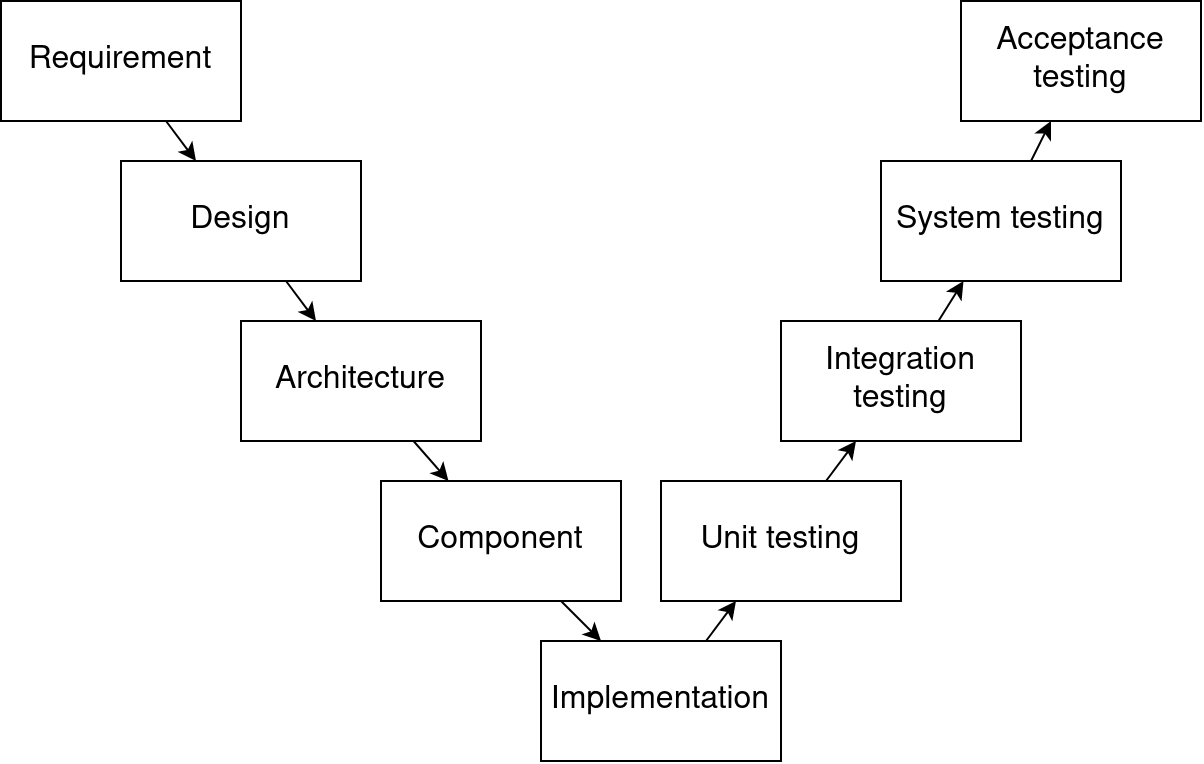
\includegraphics[width=0.5\textheight]{img/introduction/software-testing-v.drawio}
    \caption{Levels of abstraction and their corresponding tests}
    \label{fig:levels-of-abstraction-and-tests}
\end{figure}

Figure~\ref{fig:levels-of-abstraction-and-tests} describes another model, the V-model~\cite{waterfall-vs-v-model-vs-agile}.
Although in general it is considered out of date, given that agile practices are used nowadays as described before, it is helpful to visualize the layers of systems and their corresponding tests.
Single components are unit tested in isolation, while their interaction is tested using integration tests and so on and so forth.
In order to validate code before an automatic integration occurs, a well-founded set of tests is needed.
Not only on the lowest levels, but also on the highest level, which is acceptance testing.
Without strong test suits, faulty code may be integrated into a system and delivered to stakeholders.

This paper focuses on the second layer of testing, which is integration testing.
Integration testing commonly take the form of \textbf{End-to-End (E2E) testing}~\cite{end-to-end-integration-testing-design}.
As the name suggests, this technique tests a software system from one end, i.e., a hypothetical user, across user-system interaction, to the other end, i.e., the results of a feature.

For example, buying an item on an online shop can be tested using e2e tests.
First, a test program may open a browser and navigate to the website.
It then adds certain items to a cart, evaluating the shown total on the site.
It then removes and re-adds certain items while evaluating the subtotal.
After the purchase is completed, it checks that the correct entries where made in the datastore of the web shop and that all transactions were made correctly and completely.

\section{Virtualization}\label{sec:virtualization}

Some of the implementation part of this thesis is build upon Kubernetes, which is explained in section~\ref{sec:kubernetes}.
However, to effectively explain what Kubernetes is and does, containerization must be explained.
Containerization on the other hand is a subcategory of the more general field of virtualization.

\section{Kubernetes}\label{sec:kubernetes}

A large part of this thesis concerns itself with a technology called \textbf{Kubernetes}.
Kubernetes is a complex software system and care must be taken to establish different parts and concepts of it.
This section covers the basic information needed to understand how it works and what certain terminology means in its context.

First, \textbf{Images} and \textbf{Containers}\cite{docker-image} act as the base of Kubernetes.
An image can be seen as a template to a container.
It includes instructions to be run to create a container.
These instructions can range from simple commands to complex, multistep build instructions.
Any image can also serve as the starting point for a new image.
This allows the creation of complex systems that can be instantiated as containers at any time.

A container\cite{what-are-linux-containers} is a process that runs on an operating system (OS), which is mostly isolated from the host system and other processes that run on it.
In a way, they act as virtual machines.
However, they do not contain an OS themselves, but make use of the host OS through abstraction layers.
The advantage of not having to virtualize the OS is usually a better performance compared to virtual machines.
On the other hand, due to them not being completely isolated from the host OS, they have a larger impact on a system's security.

A Kubernetes system is structured as a \textbf{cluster} and therefore called a ``Kubernetes cluster''.
It is called a cluster because it is made of a cluster of \textbf{node}s.
In the context of Kubernetes, a node is computer that serves as a part of a cluster.

The smallest clusters typically have three nodes.
One control node and multiple worker nodes.
Although it is possible to have clusters with only one or two nodes, but they are mostly only used for development and debugging purposes.
Bigger clusters and clusters that are made for software systems with high availability requirements can also have multiple control nodes for redundancy.
In such cluster, worker nodes interact with one control node at a time, with other control nodes taking over if one fails.

\textbf{Pods}

\textbf{ReplicaSets}

\textbf{Deployments}

\textbf{StatefulSets}

\textbf{Side-car- or init-containers}

\textbf{Webhooks}

\textbf{Manifests}

\textbf{Helm charts}

\textbf{API}

\textbf{Operators}

\textbf{Operator Lifecycle Management (OLM)}

\textbf{AWS, GKE, and OpenShift}

\section{Similarity based variability testing}\label{sec:similarities}
As previously discussed, one of the main difficulties of testing highly scaled and complex systems, is the need of setting up complex environments.
Later it is shown, that for certain technologies, the setup for a single test may take multiple hours.
For large test suits, it is therefore unpractical to run all tests everytime, as the time-cost is too high.
In order to mitigate this issue, a technique called similarity-based variability testing is used.

Al-Hajjaji et.al., describe this technique in the context of product line testing\cite{SimilarityBasedPrioritizationInSoftwareProductLineTesting}.
A software product line is described as a base software system, which is extended with features that make use of the base system.
Due to the high variability, not all combinations and features can be practically tested.
Therefore, an algorithm is proposed, that selects tests based on similarity.

This algorithm uses a set of possible configurations, \textit{C} and a predefined definition of their similarity \textit{S} to each other\footnote{The used variable names C and S do not correspond to the variable names in the original algorithm.}.
For example, given mobile phones, two phones that both integrate a GPS transceiver are more similar to each other, than one phone that does and one that does not.
It then takes the first configuration from the input set and adds it to the result.
Then, from the selected configuration, the next, least similar, configuration is selected.
This selection is added to the result and the next, least similar, configuration to this second one is chosen.
The algorithm then continues until all configurations are sorted in the result or a limit is reached.

This algorithm, while used in a different context, is also valuable when testing complex system.
As previous discussed, for sufficiently complex environments and large test suits, not all tests can realistically be run at all times.
Analogous to configurations, metadata can also be added to define the similarity of tests to each other.
A similar algorithm as described above can then be used to sort and select tests which are possible to run in a limited timeframe.
In section \ref{sec:dynamic-testing-framework}, it is shown that this algorithm helps in implementing a solution for \textit{Q1}.

